% Options for packages loaded elsewhere
% Options for packages loaded elsewhere
\PassOptionsToPackage{unicode}{hyperref}
\PassOptionsToPackage{hyphens}{url}
%
\documentclass[
  ignorenonframetext,
  aspectratio=169,
]{beamer}
\newif\ifbibliography
\usepackage{pgfpages}
\setbeamertemplate{caption}[numbered]
\setbeamertemplate{caption label separator}{: }
\setbeamercolor{caption name}{fg=normal text.fg}
\beamertemplatenavigationsymbolsempty
% remove section numbering
\setbeamertemplate{part page}{
  \centering
  \begin{beamercolorbox}[sep=16pt,center]{part title}
    \usebeamerfont{part title}\insertpart\par
  \end{beamercolorbox}
}
\setbeamertemplate{section page}{
  \centering
  \begin{beamercolorbox}[sep=12pt,center]{section title}
    \usebeamerfont{section title}\insertsection\par
  \end{beamercolorbox}
}
\setbeamertemplate{subsection page}{
  \centering
  \begin{beamercolorbox}[sep=8pt,center]{subsection title}
    \usebeamerfont{subsection title}\insertsubsection\par
  \end{beamercolorbox}
}
% Prevent slide breaks in the middle of a paragraph
\widowpenalties 1 10000
\raggedbottom
\usepackage{iftex}
\ifPDFTeX
  \usepackage[T1]{fontenc}
  \usepackage[utf8]{inputenc}
  \usepackage{textcomp} % provide euro and other symbols
\else % if luatex or xetex
  \usepackage{unicode-math} % this also loads fontspec
  \defaultfontfeatures{Scale=MatchLowercase}
  \defaultfontfeatures[\rmfamily]{Ligatures=TeX,Scale=1}
\fi
\usepackage{lmodern}

\ifPDFTeX\else
  % xetex/luatex font selection
\fi
% Use upquote if available, for straight quotes in verbatim environments
\IfFileExists{upquote.sty}{\usepackage{upquote}}{}
\IfFileExists{microtype.sty}{% use microtype if available
  \usepackage[]{microtype}
  \UseMicrotypeSet[protrusion]{basicmath} % disable protrusion for tt fonts
}{}
\makeatletter
\@ifundefined{KOMAClassName}{% if non-KOMA class
  \IfFileExists{parskip.sty}{%
    \usepackage{parskip}
  }{% else
    \setlength{\parindent}{0pt}
    \setlength{\parskip}{6pt plus 2pt minus 1pt}}
}{% if KOMA class
  \KOMAoptions{parskip=half}}
\makeatother


\usepackage{longtable,booktabs,array}
\usepackage{calc} % for calculating minipage widths
\usepackage{caption}
% Make caption package work with longtable
\makeatletter
\def\fnum@table{\tablename~\thetable}
\makeatother
\usepackage{graphicx}
\makeatletter
\newsavebox\pandoc@box
\newcommand*\pandocbounded[1]{% scales image to fit in text height/width
  \sbox\pandoc@box{#1}%
  \Gscale@div\@tempa{\textheight}{\dimexpr\ht\pandoc@box+\dp\pandoc@box\relax}%
  \Gscale@div\@tempb{\linewidth}{\wd\pandoc@box}%
  \ifdim\@tempb\p@<\@tempa\p@\let\@tempa\@tempb\fi% select the smaller of both
  \ifdim\@tempa\p@<\p@\scalebox{\@tempa}{\usebox\pandoc@box}%
  \else\usebox{\pandoc@box}%
  \fi%
}
% Set default figure placement to htbp
\def\fps@figure{htbp}
\makeatother





\setlength{\emergencystretch}{3em} % prevent overfull lines

\providecommand{\tightlist}{%
  \setlength{\itemsep}{0pt}\setlength{\parskip}{0pt}}



 


% ============================================================
%  ECO 2203 — Beamer Metropolis Theme Preamble
%  Course: International Trade and Policy in Agriculture
%  Instructor: Nithin M, Department of Development Economics
% ============================================================

% MUST be first: load Metropolis theme before \metroset and colour overrides
\usetheme{metropolis}

% Only load packages not already provided by pandoc's beamer template
\usepackage{amsmath,amssymb}

% ---- Brand colours -----------------------------------------
\definecolor{brandblue}{HTML}{012169}
\definecolor{brandgold}{HTML}{B9975B}
\definecolor{lightblue}{HTML}{E8EDF5}

% ---- Metropolis colour overrides ---------------------------
% Main palette
\setbeamercolor{normal text}{fg=black,bg=white}
\setbeamercolor{alerted text}{fg=brandgold}
\setbeamercolor{example text}{fg=brandblue!70!black}

% Title slide
\setbeamercolor{title}{fg=white,bg=brandblue}
\setbeamercolor{subtitle}{fg=brandgold}
\setbeamercolor{author}{fg=white}
\setbeamercolor{institute}{fg=brandgold!80!white}
\setbeamercolor{date}{fg=white}
\setbeamercolor{title page header}{fg=white,bg=brandblue}

% Frametitle bar
\setbeamercolor{frametitle}{fg=white,bg=brandblue}

% Progress bar → gold
\setbeamercolor{progress bar}{fg=brandgold,bg=brandblue!30}
\setbeamercolor{title separator}{fg=brandgold}
\setbeamercolor{progress bar in head/foot}{fg=brandgold,bg=brandblue!20}
\setbeamercolor{progress bar in section page}{fg=brandgold,bg=brandblue!20}

% Blocks
\setbeamercolor{block title}{bg=brandblue,fg=white}
\setbeamercolor{block body}{bg=lightblue,fg=black}
\setbeamercolor{block title alerted}{bg=brandgold,fg=white}
\setbeamercolor{block body alerted}{bg=brandgold!12,fg=black}
\setbeamercolor{block title example}{bg=brandblue!70!black,fg=white}
\setbeamercolor{block body example}{bg=brandblue!8,fg=black}

% Structure / lists
\setbeamercolor{structure}{fg=brandblue}
\setbeamercolor{section in toc}{fg=brandblue}
\setbeamercolor{itemize item}{fg=brandblue}
\setbeamercolor{itemize subitem}{fg=brandgold}
\setbeamercolor{enumerate item}{fg=brandblue}
\setbeamercolor{description item}{fg=brandblue}

% ---- Metropolis options ------------------------------------
\metroset{
  progressbar    = frametitle,   % gold bar under frametitle
  sectionpage    = none,
  numbering      = fraction,
  block          = fill
}

% ---- Fonts (Metropolis uses Fira Sans; fallback gracefully) -
\setbeamerfont{title}{size=\Large,series=\bfseries}
\setbeamerfont{subtitle}{size=\normalsize,series=\mdseries}
\setbeamerfont{frametitle}{size=\large,series=\bfseries}
\setbeamerfont{block title}{size=\normalsize,series=\bfseries}
\setbeamerfont{caption}{size=\footnotesize}

% ---- Footer: course info + slide number --------------------
\setbeamertemplate{footline}{%
  \begin{beamercolorbox}[wd=\paperwidth,ht=2.0ex,dp=1ex]{footline}%
    \hspace{0.8em}%
    {\footnotesize\color{brandblue!60}%
      ECO 2203 \textbar{} International Trade and Policy in Agriculture
      \hfill Nithin M \hfill
      \insertframenumber{}/\inserttotalframenumber\hspace{0.8em}}%
  \end{beamercolorbox}%
}

% ---- Misc --------------------------------------------------
\setlength{\parskip}{0.25em}
\setbeamertemplate{navigation symbols}{}

% tighter column sep for side-by-side content
\setlength{\columnsep}{0.8em}

% Fix: make \label truly robust in moving arguments (Quarto generates
% \caption{\label{fig-xxx}...} which crashes Metropolis in batchmode).
% DeclareRobustCommand creates a self-protecting robust version.
\makeatletter
\let\quarto@originallabel\label
\DeclareRobustCommand*{\label}[1]{\quarto@originallabel{#1}}
\makeatother

% Prevent figures from overflowing Beamer frames.
% width=\linewidth: scale to text width (already Quarto default);
% height=0.6\textheight: cap height so figures never push past the frame bottom.
% keepaspectratio: never distort — whichever constraint binds first wins.
\setkeys{Gin}{width=\linewidth,height=0.6\textheight,keepaspectratio}
\makeatletter
\@ifpackageloaded{tcolorbox}{}{\usepackage[skins,breakable]{tcolorbox}}
\@ifpackageloaded{fontawesome5}{}{\usepackage{fontawesome5}}
\definecolor{quarto-callout-color}{HTML}{909090}
\definecolor{quarto-callout-note-color}{HTML}{0758E5}
\definecolor{quarto-callout-important-color}{HTML}{CC1914}
\definecolor{quarto-callout-warning-color}{HTML}{EB9113}
\definecolor{quarto-callout-tip-color}{HTML}{00A047}
\definecolor{quarto-callout-caution-color}{HTML}{FC5300}
\definecolor{quarto-callout-color-frame}{HTML}{acacac}
\definecolor{quarto-callout-note-color-frame}{HTML}{4582ec}
\definecolor{quarto-callout-important-color-frame}{HTML}{d9534f}
\definecolor{quarto-callout-warning-color-frame}{HTML}{f0ad4e}
\definecolor{quarto-callout-tip-color-frame}{HTML}{02b875}
\definecolor{quarto-callout-caution-color-frame}{HTML}{fd7e14}
\makeatother
\makeatletter
\@ifpackageloaded{caption}{}{\usepackage{caption}}
\AtBeginDocument{%
\ifdefined\contentsname
  \renewcommand*\contentsname{Table of contents}
\else
  \newcommand\contentsname{Table of contents}
\fi
\ifdefined\listfigurename
  \renewcommand*\listfigurename{List of Figures}
\else
  \newcommand\listfigurename{List of Figures}
\fi
\ifdefined\listtablename
  \renewcommand*\listtablename{List of Tables}
\else
  \newcommand\listtablename{List of Tables}
\fi
\ifdefined\figurename
  \renewcommand*\figurename{Figure}
\else
  \newcommand\figurename{Figure}
\fi
\ifdefined\tablename
  \renewcommand*\tablename{Table}
\else
  \newcommand\tablename{Table}
\fi
}
\@ifpackageloaded{float}{}{\usepackage{float}}
\floatstyle{ruled}
\@ifundefined{c@chapter}{\newfloat{codelisting}{h}{lop}}{\newfloat{codelisting}{h}{lop}[chapter]}
\floatname{codelisting}{Listing}
\newcommand*\listoflistings{\listof{codelisting}{List of Listings}}
\makeatother
\makeatletter
\makeatother
\makeatletter
\@ifpackageloaded{caption}{}{\usepackage{caption}}
\@ifpackageloaded{subcaption}{}{\usepackage{subcaption}}
\makeatother

\usepackage{bookmark}
\IfFileExists{xurl.sty}{\usepackage{xurl}}{} % add URL line breaks if available
\urlstyle{same}
\hypersetup{
  pdftitle={Modern Theories: Heckscher-Ohlin \& Lewis Dual-Sector Model},
  pdfauthor={Nithin M},
  hidelinks,
  pdfcreator={LaTeX via pandoc}}


\title{Modern Theories: Heckscher-Ohlin \& Lewis Dual-Sector Model}
\subtitle{ECO 2203 \textbar{} International Trade and Policy in
Agriculture}
\author{Nithin M}
\date{2026-05-23}
\institute{Department of Development Economics}

\begin{document}
\frame{\titlepage}


\section{Part I: Why Do Opportunity Costs
Differ?}\label{part-i-why-do-opportunity-costs-differ}

\begin{frame}{Recap: The Missing Piece in Ricardo}
\phantomsection\label{recap-the-missing-piece-in-ricardo}
\textbf{Last lecture:} Comparative advantage --- trade is driven by
\emph{relative} opportunity costs.

\begin{columns}[T]
\begin{column}{0.6\linewidth}
\textbf{What Ricardo established:}

\begin{itemize}
\tightlist
\item
  India has lower opportunity cost in Rice → exports Rice
\item
  World has lower opportunity cost in Wheat → exports Wheat
\item
  Both gain from specialisation and trade
\end{itemize}

\textbf{What Ricardo left unanswered:}

\begin{quote}
\emph{Why} do opportunity costs differ across countries in the first
place?
\end{quote}

Ricardo assumed labour productivity differences but gave no explanation
for \emph{why} they exist.
\end{column}

\begin{column}{0.4\linewidth}
\textbf{The Heckscher-Ohlin answer:}

Opportunity costs differ because countries differ in their
\textbf{endowments} of factors of production:

\begin{itemize}
\tightlist
\item
  Labour (\(L\))
\item
  Capital (\(K\))
\item
  Land (\(T\))
\end{itemize}

And goods differ in \textbf{factor intensity} --- how much of each
factor they require.
\end{column}
\end{columns}
\end{frame}

\begin{frame}{The Heckscher-Ohlin Framework}
\phantomsection\label{the-heckscher-ohlin-framework}
The H-O model is the workhorse of international trade theory. It
explains \emph{why} comparative advantages arise from factor abundance.

\begin{columns}[T]
\begin{column}{0.55\linewidth}
\textbf{Setup:}

\begin{itemize}
\tightlist
\item
  \textbf{Two countries:} India (\(I\)) and USA (\(U\))
\item
  \textbf{Two goods:} Rice (\(R\)) and Machines (\(M\))
\item
  \textbf{Two factors:} Labour (\(L\)) and Capital (\(K\))
\item
  Identical technologies across countries
\item
  Identical homothetic preferences
\end{itemize}

\textbf{Factor intensity definition:}

Rice is \textbf{labour-intensive} relative to Machines if:

\[\left(\frac{K}{L}\right)_R < \left(\frac{K}{L}\right)_M\]

at any common factor price ratio.
\end{column}

\begin{column}{0.45\linewidth}
\textbf{Factor abundance definition:}

India is \textbf{labour-abundant} relative to the USA if:

\[\left(\frac{K}{L}\right)^I < \left(\frac{K}{L}\right)^U\]

Equivalently, using factor prices (dual definition):

\[\left(\frac{w}{r}\right)^I < \left(\frac{w}{r}\right)^U\]

i.e., labour is \emph{relatively cheaper} in India.
\end{column}
\end{columns}
\end{frame}

\section{Part II: The Heckscher-Ohlin
Theorem}\label{part-ii-the-heckscher-ohlin-theorem}

\begin{frame}{H-O Theorem: Formal Statement}
\phantomsection\label{h-o-theorem-formal-statement}
\begin{columns}[T]
\begin{column}{0.55\linewidth}
\textbf{Theorem (Heckscher 1919; Ohlin 1933):}

\begin{quote}
A country exports the good that uses its \emph{abundant} factor
intensively.
\end{quote}

\textbf{Applied to India and USA:}

\[\left(\frac{K}{L}\right)^I < \left(\frac{K}{L}\right)^U \quad \text{(India is labour-abundant)}\]

\[\left(\frac{K}{L}\right)_R < \left(\frac{K}{L}\right)_M \quad \text{(Rice is labour-intensive)}\]

\textbf{Therefore:}

\[\text{India exports Rice; USA exports Machines}\]

\textbf{Intuition:} Labour-abundant India faces a low relative wage
\(\Rightarrow\) labour-intensive Rice is \emph{relatively cheaper} to
produce there.
\end{column}

\begin{column}{0.45\linewidth}
\textbf{Autarky prices:}

In autarky, India's abundant labour \(\Rightarrow\) low \(w/r\)
\(\Rightarrow\) low relative price of Rice:

\[\left(\frac{P_R}{P_M}\right)^I_{\text{autarky}} < \left(\frac{P_R}{P_M}\right)^U_{\text{autarky}}\]

Opening to trade raises \(P_R/P_M\) in India toward the world price:

\begin{itemize}
\tightlist
\item
  India's Rice sector expands (draws in more labour)
\item
  India's Machines sector contracts
\item
  Consistent with Rybczynski theorem (below)
\end{itemize}
\end{column}
\end{columns}
\end{frame}

\begin{frame}{The Edgeworth Box: Factor Allocation}
\phantomsection\label{the-edgeworth-box-factor-allocation}
\begin{columns}[T]
\begin{column}{0.38\linewidth}
The \textbf{Edgeworth box} shows all efficient ways to allocate
\(\bar{L}\) and \(\bar{K}\) between two sectors.

\begin{itemize}
\tightlist
\item
  Origin \(O_R\): Rice sector
\item
  Origin \(O_M\): Machines sector (rotated 180°)
\item
  \textbf{Contract curve:} locus of tangencies of Rice and Machine
  isoquants \[\frac{MPL_R}{MPK_R} = \frac{MPL_M}{MPK_M}\]
\item
  All efficient allocations lie on the contract curve
\item
  The contract curve bows toward the labour axis (Rice is
  labour-intensive)
\end{itemize}
\end{column}

\begin{column}{0.62\linewidth}
\begin{figure}

\centering{

\pandocbounded{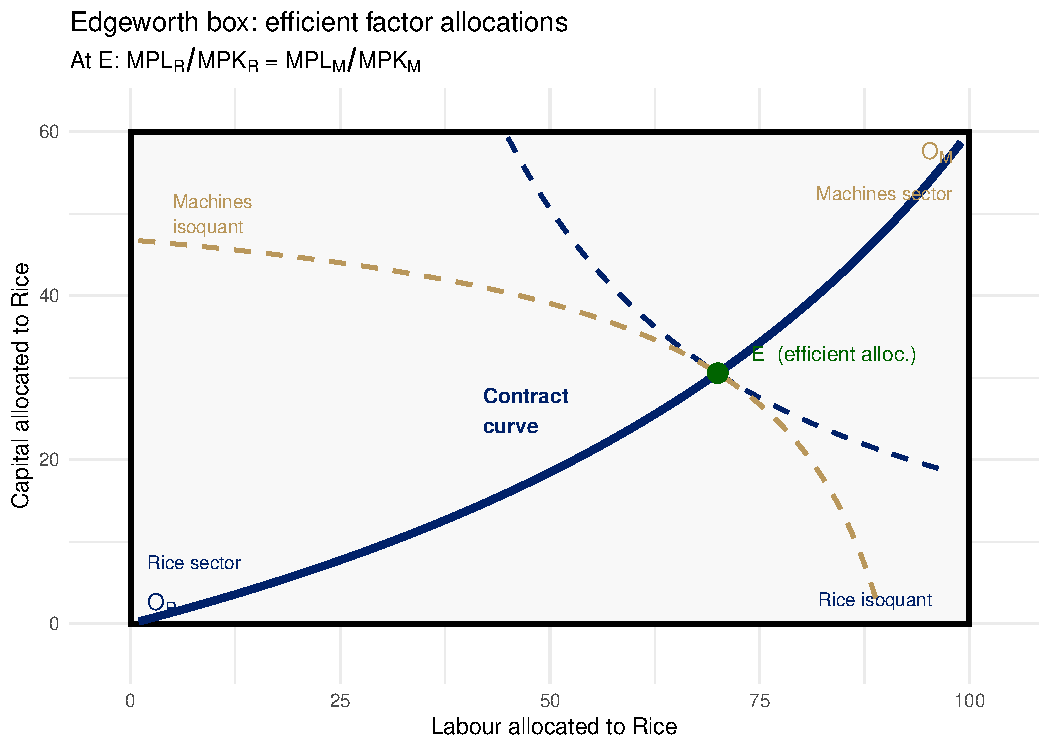
\includegraphics[keepaspectratio]{Lecture05_Modern_Theory_files/figure-beamer/fig-edgeworth-1.pdf}}

}

\caption{\label{fig-edgeworth}Edgeworth Box: Factor Allocation Between
Two Industries Source: Author's illustration.}

\end{figure}%
\end{column}
\end{columns}
\end{frame}

\begin{frame}{From Edgeworth Box to PPF}
\phantomsection\label{from-edgeworth-box-to-ppf}
The \textbf{Production Possibility Frontier} is derived from the
contract curve:

\begin{columns}[T]
\begin{column}{0.55\linewidth}
\textbf{Key insight:}

\begin{itemize}
\tightlist
\item
  Every point on the contract curve corresponds to a point on the PPF
\item
  Moving along the contract curve (reallocating factors) traces out the
  PPF
\item
  The \textbf{slope of the PPF} at any point equals the negative of the
  relative price \(P_R/P_M\)
\end{itemize}

\textbf{Factor intensity and PPF shape:}

Because Rice is labour-intensive: - Moving labour from Machines → Rice:
output of Rice rises fast (labour goes to its intensive use) - PPF is
\textbf{concave} (bowed outward) --- increasing opportunity costs

\[\frac{d^2 R}{d M^2} < 0\]

In the Ricardian model, constant labour requirements → linear PPF. H-O
gives a \emph{curved} PPF.
\end{column}

\begin{column}{0.45\linewidth}
\textbf{Illustrative PPFs:}

\pandocbounded{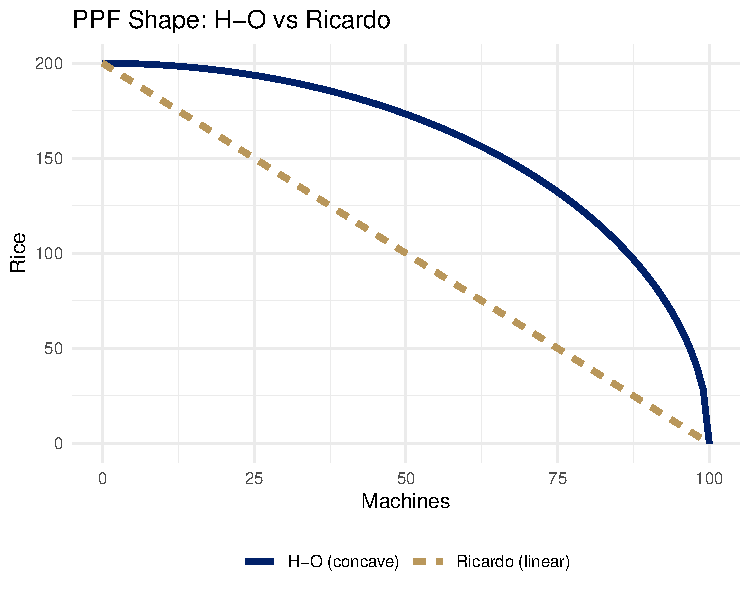
\includegraphics[keepaspectratio]{Lecture05_Modern_Theory_files/figure-beamer/unnamed-chunk-1-1.pdf}}
\end{column}
\end{columns}
\end{frame}

\section{Part III: Three Key
Theorems}\label{part-iii-three-key-theorems}

\begin{frame}{Theorem 1: Factor Price Equalisation (FPE)}
\phantomsection\label{theorem-1-factor-price-equalisation-fpe}
\textbf{Theorem (Samuelson 1948):}

Under H-O assumptions, free trade in goods \textbf{completely equalises
factor prices} across countries --- even without factor mobility:

\[w^I = w^U \qquad \text{(wages equalise)}\]
\[r^I = r^U \qquad \text{(returns to capital equalise)}\]

\textbf{Intuition:}

\begin{itemize}
\tightlist
\item
  Trade in goods is an indirect form of trading factors
\item
  India exporting Rice is equivalent to exporting embedded labour
\item
  As India expands Rice production, labour demand rises → Indian wages
  rise
\item
  As USA imports Rice, labour demand in USA Rice sector falls → US wages
  fall
\item
  In equilibrium: \(w^I = w^U\)
\end{itemize}

\begin{tcolorbox}[enhanced jigsaw, arc=.35mm, leftrule=.75mm, title=\textcolor{quarto-callout-important-color}{\faExclamation}\hspace{0.5em}{The FPE insight}, breakable, colbacktitle=quarto-callout-important-color!10!white, coltitle=black, opacityback=0, rightrule=.15mm, bottomrule=.15mm, titlerule=0mm, colback=white, bottomtitle=1mm, toprule=.15mm, left=2mm, toptitle=1mm, opacitybacktitle=0.6, colframe=quarto-callout-important-color-frame]

Free trade is a \textbf{perfect substitute} for factor mobility. This
explains why labour migration and goods trade are strategic complements
in policy debates.

\end{tcolorbox}
\end{frame}

\begin{frame}{FPE: Assumptions and Critique}
\phantomsection\label{fpe-assumptions-and-critique}
\textbf{FPE requires very strong assumptions:}

\begin{longtable}[]{@{}ll@{}}
\toprule\noalign{}
Assumption & Status in reality \\
\midrule\noalign{}
\endhead
Identical technologies & Violated (TFP gaps are large) \\
Free trade in all goods & Violated (tariffs, NTBs) \\
No factor intensity reversal & Usually holds \\
Incomplete specialisation & Often violated \\
No transport costs & Violated \\
\bottomrule\noalign{}
\end{longtable}

\textbf{Empirical reality:}

Wages in India \(\approx\) \$2/hour; USA \(\approx\) \$30/hour. FPE
clearly does \emph{not} hold in practice.

\textbf{Why study FPE then?}

\begin{itemize}
\tightlist
\item
  It reveals the \emph{forces} pushing toward convergence
\item
  Wage convergence between East Asia and OECD is partly consistent with
  FPE pressure
\item
  The direction of change (not the level) is well-predicted
\end{itemize}
\end{frame}

\begin{frame}{Theorem 2: Stolper-Samuelson Theorem}
\phantomsection\label{theorem-2-stolper-samuelson-theorem}
\textbf{Theorem (Stolper and Samuelson 1941):}

A rise in the relative price of a good raises the real return to the
factor used intensively in that good's production, and lowers the real
return to the other factor --- \textbf{more than proportionally}:

\[\hat{P}_R > 0 \Rightarrow \hat{w} > \hat{P}_R > 0 > \hat{r}\]

where \(\hat{x} \equiv d\ln x\) denotes percentage change, and Rice is
labour-intensive.

\textbf{Formal result:}

\[\hat{w} > \hat{P}_R > \hat{P}_M > \hat{r}\]

This is the \textbf{magnification effect}: factor price changes are
magnified relative to goods price changes.

\begin{columns}[T]
\begin{column}{0.5\linewidth}
\textbf{Applied to India opening to trade:}

\[P_R \uparrow \Rightarrow w \uparrow\uparrow, \quad r \downarrow\]

\begin{itemize}
\tightlist
\item
  Indian workers (abundant factor) gain
\item
  Indian capital owners (scarce factor) lose
\end{itemize}
\end{column}

\begin{column}{0.5\linewidth}
\textbf{Applied to US opening to trade:}

\[P_M \uparrow \Rightarrow r \uparrow\uparrow, \quad w \downarrow\]

\begin{itemize}
\tightlist
\item
  US capital owners gain
\item
  US workers lose → \textbf{political economy of protectionism!}
\end{itemize}
\end{column}
\end{columns}
\end{frame}

\begin{frame}{Stolper-Samuelson: Policy Relevance}
\phantomsection\label{stolper-samuelson-policy-relevance}
\begin{columns}[T]
\begin{column}{0.55\linewidth}
\textbf{Why does Stolper-Samuelson matter for policy?}

It explains \emph{who lobbies for and against trade liberalisation}:

\begin{itemize}
\tightlist
\item
  Labour in labour-abundant countries → \textbf{pro-trade}
\item
  Capital in labour-abundant countries → \textbf{anti-trade} (or
  sector-specific)
\item
  Labour in capital-abundant countries → \textbf{anti-trade} (e.g., US
  manufacturing unions)
\item
  Capital in capital-abundant countries → \textbf{pro-trade}
\end{itemize}

\textbf{India's agricultural trade policy:}

When India raises rice export prices via MSP increases:

\[P_R \uparrow \Rightarrow w_{\text{agri}} \uparrow \Rightarrow \text{rural wages rise}\]

This is Stolper-Samuelson in action --- higher output prices benefit
agricultural labour.
\end{column}

\begin{column}{0.45\linewidth}
\textbf{The compensation principle:}

Even when aggregate welfare rises, there are \textbf{distributional
losers}.

A country could in principle use the gains to compensate losers, but in
practice:

\begin{enumerate}
\tightlist
\item
  Compensation schemes are costly to administer
\item
  Political constraints prevent redistribution
\item
  Short-run adjustment costs fall unevenly
\end{enumerate}

This is why \textbf{trade adjustment assistance} (TAA) programs exist in
many countries.
\end{column}
\end{columns}
\end{frame}

\begin{frame}{Theorem 3: Rybczynski Theorem}
\phantomsection\label{theorem-3-rybczynski-theorem}
\textbf{Theorem (Rybczynski 1955):}

At constant goods prices, an increase in the endowment of a factor
causes:

\[L \uparrow \Rightarrow Q_R \uparrow\uparrow \text{ and } Q_M \downarrow\]

More precisely:

\[\hat{Q}_R > \hat{L} > 0 > \hat{Q}_M\]

\begin{itemize}
\tightlist
\item
  Output of the labour-intensive good rises \textbf{more than
  proportionally} to the labour increase
\item
  Output of the capital-intensive good \textbf{falls absolutely}
\end{itemize}

\begin{columns}[T]
\begin{column}{0.5\linewidth}
\textbf{Intuition:}

Expanding Rice output (to absorb new labour) requires withdrawing
capital from Machines, even though capital endowment is unchanged. At
constant prices, the only way to re-equate factor ratios is to pull
capital into Rice and contract Machines.
\end{column}

\begin{column}{0.5\linewidth}
\textbf{India application:}

India's rural-to-urban migration (labour inflow to manufacturing) can be
seen as a Rybczynski effect in reverse:

\[L_{\text{mfg}} \uparrow \Rightarrow Q_{\text{mfg}} \uparrow\uparrow, \quad Q_{\text{agri}} \downarrow\]

Structural transformation is partly a Rybczynski phenomenon.
\end{column}
\end{columns}
\end{frame}

\begin{frame}{Rybczynski Effect: PPF Diagram}
\phantomsection\label{rybczynski-effect-ppf-diagram}
\begin{columns}[T]
\begin{column}{0.4\linewidth}
An inflow of labour \textbf{rotates} the PPF outward, but
asymmetrically:

\begin{itemize}
\tightlist
\item
  The Rice (labour-intensive) intercept expands greatly
\item
  The Machines (capital-intensive) intercept contracts
\end{itemize}

At the \textbf{original price ratio}, the economy moves from A to B:

\begin{itemize}
\tightlist
\item
  More Rice produced (\(Q_R \uparrow\uparrow\))
\item
  Fewer Machines (\(Q_M \downarrow\))
\end{itemize}

This is the \textbf{Rybczynski line} --- locus of output combinations at
constant prices as labour endowment varies.
\end{column}

\begin{column}{0.6\linewidth}
\begin{figure}

\centering{

\pandocbounded{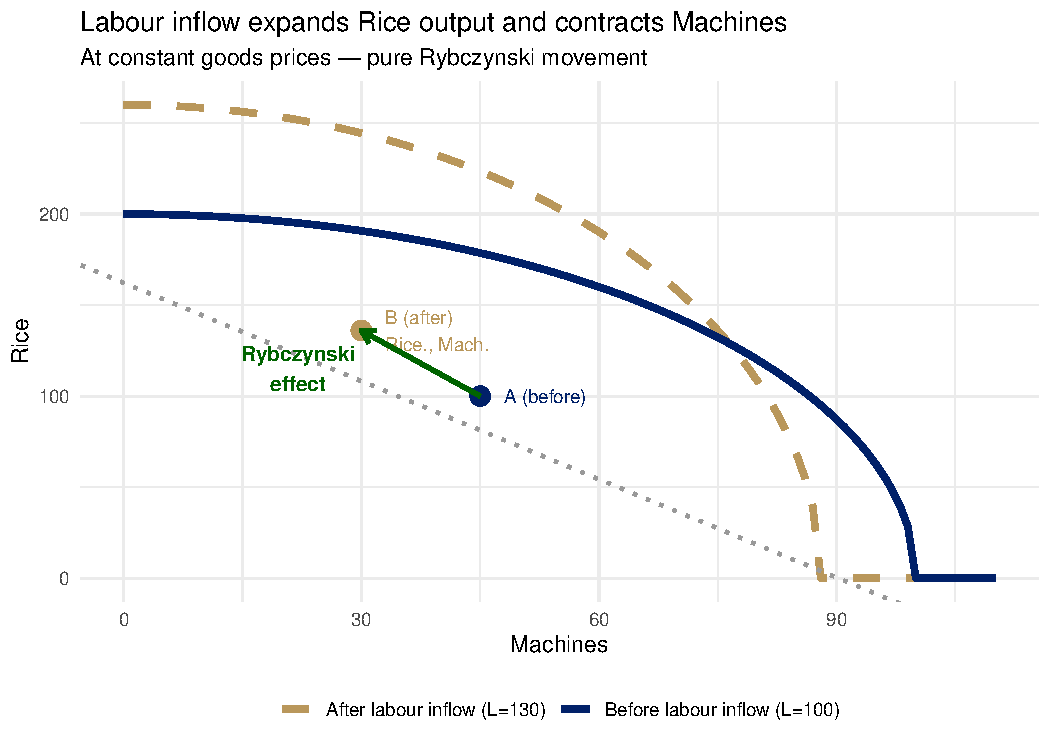
\includegraphics[keepaspectratio]{Lecture05_Modern_Theory_files/figure-beamer/fig-rybczynski-1.pdf}}

}

\caption{\label{fig-rybczynski}Rybczynski Effect: Labour Inflow Shifts
PPF Source: Author's illustration.}

\end{figure}%
\end{column}
\end{columns}
\end{frame}

\section{Part IV: The Leontief Paradox and
Extensions}\label{part-iv-the-leontief-paradox-and-extensions}

\begin{frame}{The Leontief Paradox (1953)}
\phantomsection\label{the-leontief-paradox-1953}
\textbf{The test:} Wassily Leontief (1953) used US input-output tables
to measure the capital and labour content of US exports and imports.

\textbf{The prediction (H-O):} The USA, being capital-abundant, should
export capital-intensive goods and import labour-intensive goods.

\textbf{The finding:} US exports were \emph{more labour-intensive} than
US imports --- \textbf{the opposite of H-O!}

\textbf{Formal statement of the paradox:}

\[\left(\frac{K}{L}\right)_{\text{US exports}} < \left(\frac{K}{L}\right)_{\text{US imports}}\]

This contradicts the basic H-O prediction for a capital-abundant
country.
\end{frame}

\begin{frame}{Factor Intensity of India's Trade}
\phantomsection\label{factor-intensity-of-indias-trade}
\begin{figure}

\centering{

\pandocbounded{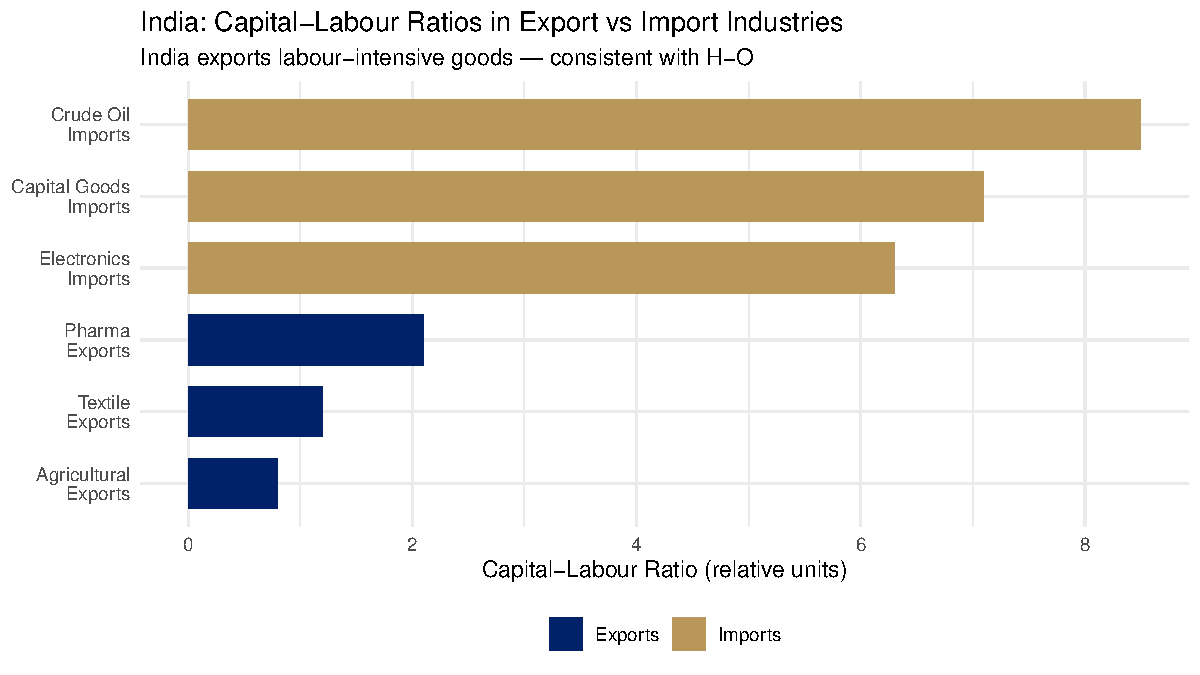
\includegraphics[keepaspectratio]{Lecture05_Modern_Theory_files/figure-beamer/fig-leontief-1.pdf}}

}

\caption{\label{fig-leontief}Factor Intensity of India's Exports vs
Imports (illustrative) Source: Author's illustration based on DGCI\&S /
World Bank data.}

\end{figure}%

\textbf{India does NOT exhibit a Leontief paradox} --- it exports
labour-intensive goods, consistent with H-O.
\end{frame}

\begin{frame}{Explanations for the Leontief Paradox}
\phantomsection\label{explanations-for-the-leontief-paradox}
Several resolutions have been proposed:

\begin{columns}[T]
\begin{column}{0.55\linewidth}
\textbf{1. Human capital:}

US labour is highly skilled --- skill-adjusted, US workers embody large
amounts of human capital. US exports are ``labour-intensive'' in
unskilled labour but capital-intensive in human capital.

\[\text{Effective } K/L = \frac{K + K_H}{L}\]

\textbf{2. Factor intensity reversals:}

Same good can be labour-intensive in one country and capital-intensive
in another (different factor prices → different techniques).

\textbf{3. Natural resource abundance:}

US imports include oil and raw materials --- these are
capital-intensive. Excluding natural resource industries resolves much
of the paradox.
\end{column}

\begin{column}{0.45\linewidth}
\textbf{4. Demand bias:}

US consumers have stronger preference for capital-intensive goods (high
income elasticity of demand for manufactures). Demand effects can offset
supply-side comparative advantage.

\textbf{5. Trade barriers:}

US tariff structure historically protected labour-intensive industries
(agriculture, textiles), distorting trade flows away from comparative
advantage.

\textbf{Modern verdict (Trefler 1995):}

Allowing for \textbf{technology differences} and \textbf{factor
productivity} differences across countries reconciles most of the H-O
predictions with data --- the ``mystery of the missing trade'' is partly
resolved.
\end{column}
\end{columns}
\end{frame}

\section{Part V: The Lewis Dual-Sector Model and Agricultural
Trade}\label{part-v-the-lewis-dual-sector-model-and-agricultural-trade}

\begin{frame}{Lewis (1954): Structural Transformation}
\phantomsection\label{lewis-1954-structural-transformation}
While H-O focuses on \emph{between-country} differences, the
\textbf{Lewis model} explains how factor endowments evolve \emph{within}
a developing country:

\begin{columns}[T]
\begin{column}{0.55\linewidth}
\textbf{Two sectors:}

\begin{itemize}
\tightlist
\item
  \textbf{Traditional sector (agriculture):} large labour surplus, low
  marginal product of labour (\(MPL_A \approx 0\))
\item
  \textbf{Modern sector (industry/services):} rising capital intensity,
  higher wages
\end{itemize}

\textbf{Lewis's key assumption:}

\[MPL_A < \bar{w}_{\text{subsistence}}\]

There is a pool of ``surplus labour'' in agriculture that can be
absorbed by industry \textbf{without raising agricultural wages}.

\textbf{Migration condition:}

Workers migrate from agriculture to industry as long as:

\[w_{\text{industry}} > w_{\text{agriculture}}\]
\end{column}

\begin{column}{0.45\linewidth}
\textbf{Implications for agricultural trade:}

During the Lewis transition:

\begin{enumerate}
\tightlist
\item
  Agricultural labour supply is highly elastic → low rural wages
\item
  Low wages → comparative advantage in labour-intensive agricultural
  exports
\item
  As industrialisation proceeds → rural wages rise → agricultural
  comparative advantage erodes
\item
  Eventually: Rybczynski-type shift away from agricultural exports
\end{enumerate}

\textbf{East Asia's trajectory:}

Japan (1950s--70s) → South Korea (1970s--90s) → China (2000s--) each
followed this path: strong agricultural/labour-intensive exports early,
shifting to capital-intensive manufactures.
\end{column}
\end{columns}
\end{frame}

\begin{frame}{Lewis Model: Diagrammatic Analysis}
\phantomsection\label{lewis-model-diagrammatic-analysis}
\begin{figure}

\centering{

\pandocbounded{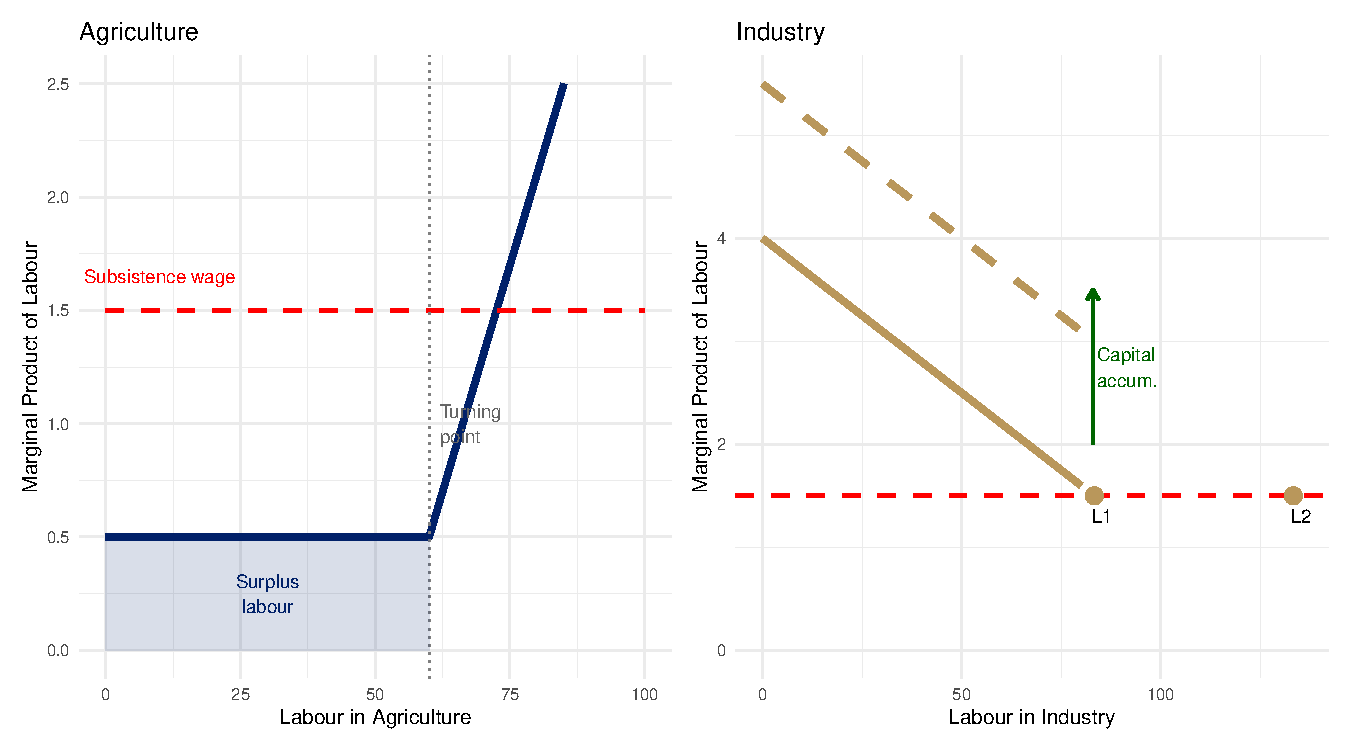
\includegraphics[keepaspectratio]{Lecture05_Modern_Theory_files/figure-beamer/fig-lewis-1.pdf}}

}

\caption{\label{fig-lewis}Lewis Model: Surplus Labour Transfer and
Structural Transformation Source: Author's illustration after Lewis
(1954).}

\end{figure}%
\end{frame}

\begin{frame}{H-O, Lewis, and India's Agricultural Exports}
\phantomsection\label{h-o-lewis-and-indias-agricultural-exports}
\begin{columns}[T]
\begin{column}{0.55\linewidth}
\textbf{Connecting the models:}

\begin{longtable}[]{@{}
  >{\raggedright\arraybackslash}p{(\linewidth - 4\tabcolsep) * \real{0.3333}}
  >{\raggedright\arraybackslash}p{(\linewidth - 4\tabcolsep) * \real{0.3333}}
  >{\raggedright\arraybackslash}p{(\linewidth - 4\tabcolsep) * \real{0.3333}}@{}}
\toprule\noalign{}
\begin{minipage}[b]{\linewidth}\raggedright
Mechanism
\end{minipage} & \begin{minipage}[b]{\linewidth}\raggedright
H-O
\end{minipage} & \begin{minipage}[b]{\linewidth}\raggedright
Lewis
\end{minipage} \\
\midrule\noalign{}
\endhead
Source of CA & Factor endowments & Wage dualism \\
Key variable & \(K/L\) ratio & \(MPL_A\) vs \(\bar{w}\) \\
Trade prediction & Export labour-intensive goods & Export goods with
surplus-labour content \\
Dynamics & Static & Dynamic (transition) \\
\bottomrule\noalign{}
\end{longtable}

\textbf{Combined implication for India:}

India currently sits at an early Lewis stage:

\begin{itemize}
\tightlist
\item
  Large agricultural labour surplus (\(\approx 40\)\% of workforce in
  agriculture)
\item
  Low rural wages → strong comparative advantage in labour-intensive
  agri exports
\item
  As structural transformation proceeds, advantage will erode (as it did
  in South Korea)
\end{itemize}
\end{column}

\begin{column}{0.45\linewidth}
\textbf{India's agricultural export performance (FY2024):}

\begin{itemize}
\tightlist
\item
  Total agri-food exports: \textbf{\$43.7 billion}
\item
  Rice: \(\approx\) \$10.4 billion (before export ban)
\item
  Marine products: \$7.6 billion
\item
  Spices: \$3.7 billion
\item
  Cotton: \$2.1 billion
\end{itemize}

\textbf{H-O explains:} labour-intensive crops dominate

\textbf{Lewis explains:} low rural wages underpin price competitiveness

\textbf{Policy implication:} India should invest in agricultural
productivity to maintain competitiveness even as wages rise --- moving
up the value chain rather than defending low-wage advantage.
\end{column}
\end{columns}
\end{frame}

\section{Part VI: Summary and Looking
Ahead}\label{part-vi-summary-and-looking-ahead}

\begin{frame}{The Modern Theory of Trade: Summary}
\phantomsection\label{the-modern-theory-of-trade-summary}
\begin{columns}[T]
\begin{column}{0.5\linewidth}
\textbf{Three pillars of the H-O framework:}

\begin{enumerate}
\item
  \textbf{H-O Theorem:} countries export goods intensive in their
  abundant factor
\item
  \textbf{Factor Price Equalisation:} \[w^I = w^U, \quad r^I = r^U\]
  (free trade substitutes for factor mobility)
\item
  \textbf{Stolper-Samuelson:}
  \[\hat{P}_R > 0 \Rightarrow \hat{w} > \hat{P}_R > 0 > \hat{r}\] (trade
  has stark distributional effects)
\item
  \textbf{Rybczynski:}
  \[\hat{L} > 0 \Rightarrow \hat{Q}_R > \hat{L} > 0 > \hat{Q}_M\]
  (factor accumulation biases production)
\end{enumerate}
\end{column}

\begin{column}{0.5\linewidth}
\textbf{Empirical scorecard:}

\begin{longtable}[]{@{}ll@{}}
\toprule\noalign{}
Prediction & Evidence \\
\midrule\noalign{}
\endhead
Factor content of trade & Mixed (Trefler 1995) \\
India exports labour-intensive & Confirmed \\
Wage convergence & Partial (direction correct) \\
Stolper-Samuelson effects & Strong in long run \\
Rybczynski (structural change) & Strong (East Asia) \\
\bottomrule\noalign{}
\end{longtable}

\textbf{What H-O cannot explain:}

\begin{itemize}
\tightlist
\item
  Intra-industry trade (Germany ↔ France in cars)
\item
  Trade between similar countries
\item
  Scale economies and first-mover advantages → \textbf{New Trade Theory}
  (Lecture 6): Krugman (1979), Helpman-Krugman (1985)
\end{itemize}
\end{column}
\end{columns}
\end{frame}

\begin{frame}{Looking Ahead: New Trade Theory}
\phantomsection\label{looking-ahead-new-trade-theory}
\textbf{Why do we need a theory beyond H-O?}

\begin{itemize}
\tightlist
\item
  \(\approx 60\%\) of world trade is \textbf{intra-industry} (exchanging
  similar goods)
\item
  Large share of trade is \textbf{between similar, high-income
  countries}
\item
  \textbf{Scale economies} matter --- firms, not just countries, have
  comparative advantages
\end{itemize}

\textbf{Krugman's (1979) insight:}

Even with identical factor endowments, countries gain from trade
because:

\[\text{Specialisation} \Rightarrow \text{Scale economies} \Rightarrow \text{Lower costs} \Rightarrow \text{More variety}\]

Each country specialises in a \emph{different} variety of the same good
--- gains arise from \textbf{love of variety}, not factor endowments.

\textbf{Next lecture:} Economies of scale, monopolistic competition, and
the new economic geography --- why do trade and production cluster? And
what does this mean for India's agricultural processing sector? :::
\end{frame}

\section{Appendix}\label{appendix}

\begin{frame}{Additional Resources}
\phantomsection\label{additional-resources}
\begin{columns}[T]
\begin{column}{0.5\linewidth}
\textbf{Further Reading}

\begin{itemize}
\tightlist
\item
  \emph{International Economics} --- Salvatore (Ch. 4-5)
\item
  \emph{International Economics} --- Appleyard \& Field (Ch. 4-5)
\item
  RBI/DGCI\&S/APEDA databases for latest data
\end{itemize}
\end{column}

\begin{column}{0.5\linewidth}
\textbf{Key Data Sources}

\begin{itemize}
\tightlist
\item
  DGCI\&S: India's merchandise trade
\item
  RBI: Balance of payments data\\
\item
  APEDA: Agricultural export statistics
\item
  WTO: Tariff and trade databases
\end{itemize}
\end{column}
\end{columns}
\end{frame}




\end{document}
